\section{Fourierreihe}
Komplex:
\begin{equation}
\nonumber
\boxed{f(t) = \sum\limits_{k = -\infty}^{\infty} c_k \cdot e^{j k  	\omega_f t}}= \sum\limits_{k = 0}^{\infty} \left(c_k \cdot e^{j k \omega_f t} + \overline{c_k} \cdot e^{-j k \omega_f t}\right) \quad  \boxed{c_k=\overline{c_{-k}}=\frac{1}{T}\int_0^T{f(t)\cdot 	e^{-jk\omega_f t}dt}}
\end{equation}
	
\vspace{0.5cm}

Reell:
\[
\boxed{f(t) = \frac{a_0}{2} + \sum\limits_{k=1}^{\infty} \left[a_k \cos(k \omega_f t) + b_k \sin(k \omega_f t)\right]}=\frac{A_0}{2} + \sum\limits_{k=1}^{\infty} A_k \cos(k\omega_f t + \varphi_k) \quad k\in
  	\mathbb{Z}
\]	
	
\[\boxed{a_0 =
	\frac{2}{T}\int\limits_0^{T} f(t)dt, \quad a_k = \frac{2}{T}\int\limits_0^{T} f(t)\cos(k \omega_f t) dt, \quad b_k =
	\frac{2}{T}\int\limits_0^{T} f(t)\sin(k \omega_f t) dt} \quad
	\omega_f=\frac{2 \pi}{T}=2 \pi f
\]
	
\vspace{0.5cm}

$a_0$, $c_0$, $A_0$ sind \textit{Konstanten}, $\omega_f$ ist die \textit{Grundkreisfrequenz}, $a_k$ und $b_k$ sind die \textit{reellen Koeffizienten}, 
$c_k$ ist der \textit{komplexe Koeffizient}, $A_k$ ist die \textit{Amplitude} und $\varphi_k$ ist die \textit{Phase}.

\begin{tabular}{p{9cm}p{9cm}}
  $a_k = c_k + \bar{c_k} = 2 \text{Re}(c_k) = A_k \cos(\varphi_k)$ &
  $b_k = j(c_k + \bar{c_k}) = -2 \text{Im}(c_k) = -A_k \sin(\varphi_k)$ \\
  $c_k = \frac{a_k-jb_k}{2} = \frac{A_k}{2} e^{j\varphi_k}$ &
  $c_{-k} = \overline{c_k} = \frac{a_k+jb_k}{2} = \frac{A_k}{2} e^{-j\varphi_k}$ \\
  $A_k = 2|c_k| = \sqrt{a_k^2+b_k^2}$
\end{tabular}

\vspace{0.5cm}

Berechnung von $\varphi_k$ aus $a_k$ und $b_k$:\\
\begin{tabular}{p{2.5cm}p{3.5cm}p{2cm}p{2.5cm}p{3.5cm}}
	$a_k> 0:$ & $\varphi_k = -\arctan(\frac{b_k}{a_k})$ & &
	$a_k<0:$ &	$\varphi_k = -\arctan(\frac{b_k}{a_k}) + \pi$\\
	%\hline
	$a_k = 0; b_k > 0:$ &	$\varphi_k = -\frac{\pi}{2}$ & &
	$a_k = 0; b_k < 0:$ &	$\varphi_k = \frac{\pi}{2}$\\
	%\hline
	$a_k = b_k = 0:$ &	$\varphi_k = \text{nicht definiert}$ & & & $\varphi_k =
	arg(c_k)$
\end{tabular}

\subsection{Symmetrie}
\begin{tabular}{|p{4.3cm}|p{4.3cm}|p{4.3cm}|p{4.3cm}|}
  \hline
 	\textbf{gerade Funktion} & \textbf{ungerade Funktion} &
 	\textbf{Halbperiode 1} & \textbf{Halbperiode 2}\\
 	%\hline
 	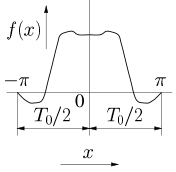
\includegraphics[width=3cm]{content/appendix/geradeFunktion.png}&
 	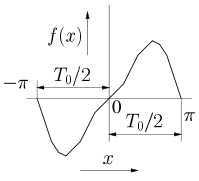
\includegraphics[width=3cm]{content/appendix/ungeradeFunktion.png}&   
  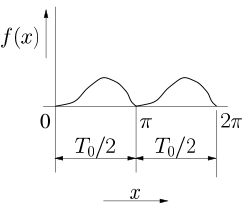
\includegraphics[width=3cm]{content/appendix/halbperiode1.png}&   
  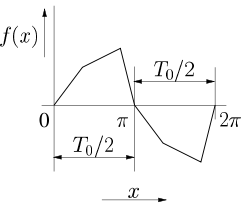
\includegraphics[width=3cm]{content/appendix/halbperiode2.png}\\
	& & & \\			
	$f(-t)=f(t)$ & $f(-t)=-f(t)$ & $f(t)=f(t+\pi)$ & $f(t)=-f(t+\pi)$\\
	$b_k=0$ & $a_k=0$ & $a_{2k+1}=0$ & $a_{2k}=0$\\
	$a_k = \frac{4}{T} \int\limits_0^{\frac{T}{2}} f(t) \cdot \cos(k \omega_f
	t) dt$ &
	$b_k =  \frac{4}{T} \int\limits_0^{\frac{T}{2}} f(t) \cdot
  \sin(k \omega_f t) dt$ &
	$b_{2k+1}=0$ & $b_{2k}=0$\\
	\hline
\end{tabular} 
    
     	
\subsection{Spektren}

\begin{tabular}{p{0.3\textwidth}p{0.3\textwidth}p{0.3\textwidth}}
	Kosinus- Sinusamplitudenspek. & 
	Einseitiges Ampl.-/ Phasenspek. &
	Zweiseitiges Ampl.-/ Phasenspek. \\
	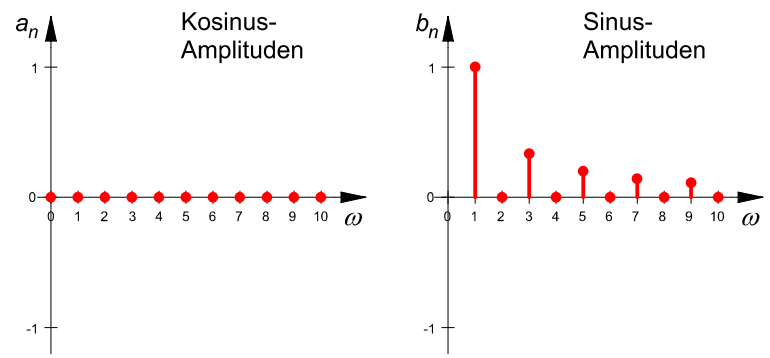
\includegraphics[width=5cm]{content/appendix/cosSinSpectr.png} &
	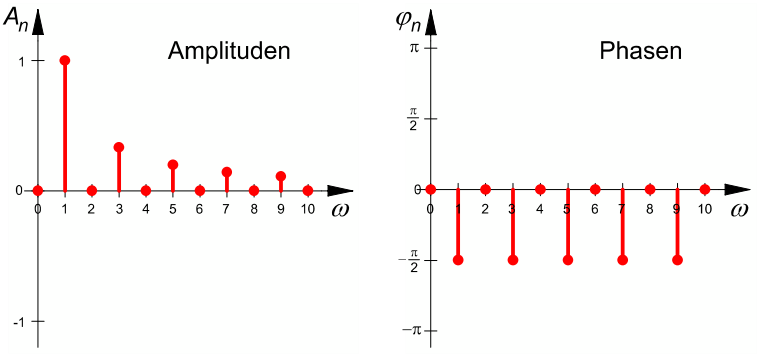
\includegraphics[width=5cm]{content/appendix/EinseitigSpectr.png} &
	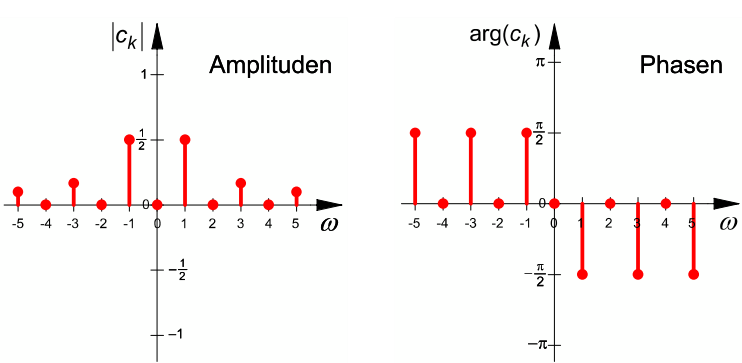
\includegraphics[width=5cm]{content/appendix/ZweiseitigSpectr.png}
\end{tabular}

Das einseitige und zweiseitige Spektrum unterscheiden sich nur im
Amplitudendiagramm. Das Phasendiagramm für positive $k$ ist identisch. Die
Amplitudenwerte sind hälftig auf die pos. und neg. $k$ verteilt.

\subsection{Rechenregeln}
\begin{tabular}{p{0.25\textwidth}p{0.25\textwidth}p{0.25\textwidth}p{0.25\textwidth}}
  Ableiten & $\frac{\text{d}}{\text{d}t}\sum c_n \e^{j\omega_0 n t}=\sum c_n' \e^{j \omega_0 n t}$ & $c_n'=j\omega_0 n c_n$ & $\omega_0 = \frac{2 \pi}{T}$ \\
  Integrieren & $\int \sum c_n \e^{j\omega_0 n t} = \sum \tilde{c_{n}} \e^{j\omega_0 n t}$ & $\tilde{c_n}=\frac{1}{j\omega_0 n}c_n$ & $n\neq 0$ \\
  Verschieben & $s(t) = \sum c_n \e^{j\omega_0 n t}$ & $s(t-\tau)=\sum c_{n\tau}\e^{j\omega_0 n t}$ & $c_{n\tau}=c_n \e^{-j\omega_0 n \tau}$
\end{tabular}
